%% BioMed_Central_Tex_Template_v1.06
%%                                      %
%  bmc_article.tex            ver: 1.06 %
%                                       %

%%IMPORTANT: do not delete the first line of this template
%%It must be present to enable the BMC Submission system to
%%recognise this template!!

%%%%%%%%%%%%%%%%%%%%%%%%%%%%%%%%%%%%%%%%%
%%                                     %%
%%  LaTeX template for BioMed Central  %%
%%     journal article submissions     %%
%%                                     %%
%%          <8 June 2012>              %%
%%                                     %%
%%                                     %%
%%%%%%%%%%%%%%%%%%%%%%%%%%%%%%%%%%%%%%%%%


%%%%%%%%%%%%%%%%%%%%%%%%%%%%%%%%%%%%%%%%%%%%%%%%%%%%%%%%%%%%%%%%%%%%%
%%                                                                 %%
%% For instructions on how to fill out this Tex template           %%
%% document please refer to Readme.html and the instructions for   %%
%% authors page on the biomed central website                      %%
%% http://www.biomedcentral.com/info/authors/                      %%
%%                                                                 %%
%% Please do not use \input{...} to include other tex files.       %%
%% Submit your LaTeX manuscript as one .tex document.              %%
%%                                                                 %%
%% All additional figures and files should be attached             %%
%% separately and not embedded in the \TeX\ document itself.       %%
%%                                                                 %%
%% BioMed Central currently use the MikTex distribution of         %%
%% TeX for Windows) of TeX and LaTeX.  This is available from      %%
%% http://www.miktex.org                                           %%
%%                                                                 %%
%%%%%%%%%%%%%%%%%%%%%%%%%%%%%%%%%%%%%%%%%%%%%%%%%%%%%%%%%%%%%%%%%%%%%

%%% additional documentclass options:
%  [doublespacing]
%  [linenumbers]   - put the line numbers on margins

%%% loading packages, author definitions

%\documentclass[twocolumn]{bmcart}% uncomment this for twocolumn layout and comment line below
\documentclass{bmcart}

%%% Load packages
%\usepackage{amsthm,amsmath}
%\RequirePackage{natbib}
\RequirePackage{hyperref}
\usepackage[utf8]{inputenc} %unicode support
\usepackage{graphicx}
\usepackage{setspace}
\usepackage[T1]{fontenc}
%\usepackage[applemac]{inputenc} %applemac support if unicode package fails
%\usepackage[latin1]{inputenc} %UNIX support if unicode package fails


%%%%%%%%%%%%%%%%%%%%%%%%%%%%%%%%%%%%%%%%%%%%%%%%%
%%                                             %%
%%  If you wish to display your graphics for   %%
%%  your own use using includegraphic or       %%
%%  includegraphics, then comment out the      %%
%%  following two lines of code.               %%
%%  NB: These line *must* be included when     %%
%%  submitting to BMC.                         %%
%%  All figure files must be submitted as      %%
%%  separate graphics through the BMC          %%
%%  submission process, not included in the    %%
%%  submitted article.                         %%
%%                                             %%
%%%%%%%%%%%%%%%%%%%%%%%%%%%%%%%%%%%%%%%%%%%%%%%%%


%\def\includegraphic{}
%\def\includegraphics{}



%%% Put your definitions there:
\startlocaldefs
\endlocaldefs


%%% Begin ...
\begin{document}

%%% Start of article front matter
\begin{frontmatter}

\begin{fmbox}
\dochead{Research}

%%%%%%%%%%%%%%%%%%%%%%%%%%%%%%%%%%%%%%%%%%%%%%
%%                                          %%
%% Enter the title of your article here     %%
%%                                          %%
%%%%%%%%%%%%%%%%%%%%%%%%%%%%%%%%%%%%%%%%%%%%%%

\title{Mimoza: Web-Based Semantic Zooming and Navigation in Metabolic Networks}

%%%%%%%%%%%%%%%%%%%%%%%%%%%%%%%%%%%%%%%%%%%%%%
%%                                          %%
%% Enter the authors here                   %%
%%                                          %%
%% Specify information, if available,       %%
%% in the form:                             %%
%%   <key>={<id1>,<id2>}                    %%
%%   <key>=                                 %%
%% Comment or delete the keys which are     %%
%% not used. Repeat \author command as much %%
%% as required.                             %%
%%                                          %%
%%%%%%%%%%%%%%%%%%%%%%%%%%%%%%%%%%%%%%%%%%%%%%

\author[
   addressref={aff1},                   % id's of addresses, e.g. {aff1,aff2}
   corref={aff1},                       % id of corresponding address, if any
   %noteref={n1},                        % id's of article notes, if any
   email={anna.zhukova@inria.fr}   % email address
]{\inits{AZ}\fnm{Anna} \snm{Zhukova}}
\author[
   addressref={aff1},
   email={david.sherman@inria.fr}
]{\inits{DJS}\fnm{David J} \snm{Sherman}}

%%%%%%%%%%%%%%%%%%%%%%%%%%%%%%%%%%%%%%%%%%%%%%
%%                                          %%
%% Enter the authors' addresses here        %%
%%                                          %%
%% Repeat \address commands as much as      %%
%% required.                                %%
%%                                          %%
%%%%%%%%%%%%%%%%%%%%%%%%%%%%%%%%%%%%%%%%%%%%%%

\address[id=aff1]{%                           % unique id
  \orgname{Inria/Universit\'e Bordeaux/CNRS joint project-team MAGNOME}, % university, etc
  \street{351, cours de la Lib\'{e}ration},                     %
  \postcode{F-33405}                                % post or zip code
  \city{Talence},                              % city
  \cny{France}                                    % country
}

%%%%%%%%%%%%%%%%%%%%%%%%%%%%%%%%%%%%%%%%%%%%%%
%%                                          %%
%% Enter short notes here                   %%
%%                                          %%
%% Short notes will be after addresses      %%
%% on first page.                           %%
%%                                          %%
%%%%%%%%%%%%%%%%%%%%%%%%%%%%%%%%%%%%%%%%%%%%%%

\begin{artnotes}
%\note{Sample of title note}     % note to the article
%\note[id=n1]{Equal contributor} % note, connected to author
\end{artnotes}

\end{fmbox}% comment this for two column layout

%%%%%%%%%%%%%%%%%%%%%%%%%%%%%%%%%%%%%%%%%%%%%%
%%                                          %%
%% The Abstract begins here                 %%
%%                                          %%
%% Please refer to the Instructions for     %%
%% authors on http://www.biomedcentral.com  %%
%% and include the section headings         %%
%% accordingly for your article type.       %%
%%                                          %%
%%%%%%%%%%%%%%%%%%%%%%%%%%%%%%%%%%%%%%%%%%%%%%

\begin{abstractbox}

\begin{abstract} % abstract

\parttitle{Motivation}
The complexity of genome-scale metabolic models makes them quite difficult for human users to read, since they contain thousands of reactions that must be included for accurate computer simulation. For example, the metabolic network of the bacterium \emph{E. coli} contains 2\,168 reactions, the \emph{yeast 7} metabolic network model of \emph{S.~cerevisiae} includes 2\,352 reactions, and \emph{recon 2}, a global human metabolism reconstruction, has 7\,440 reactions. Interestingly, hidden similarities between groups of reactions can be discovered, and generalized to reveal higher-level patterns.

\parttitle{Results}
The web-based navigation system Mimoza allows a human expert to explore metabolic models in a semantically zoomable manner: The most general view represents the compartments of the model; the next view shows the generalized versions of reactions and metabolites in each compartment; and the most detailed view represents the initial model with the generalization-based layout (where similar metabolites and reactions are placed next to each other). It allows a human expert to grasp the general structure of the model and analyze it in a top-down manner.
Mimoza can be installed standalone, or used on-line at http://mimoza.bordeaux.inria.fr/, or installed in a Galaxy server for use in workflows.
Mimoza views can be embedded in web pages, or downloaded as COMBINE archives.
\end{abstract}

%%%%%%%%%%%%%%%%%%%%%%%%%%%%%%%%%%%%%%%%%%%%%%
%%                                          %%
%% The keywords begin here                  %%
%%                                          %%
%% Put each keyword in separate \kwd{}.     %%
%%                                          %%
%%%%%%%%%%%%%%%%%%%%%%%%%%%%%%%%%%%%%%%%%%%%%%

\begin{keyword}
\kwd{metabolic modeling}
\kwd{visualization}
\kwd{model generalization}
\end{keyword}

% MSC classifications codes, if any
%\begin{keyword}[class=AMS]
%\kwd[Primary ]{}
%\kwd{}
%\kwd[; secondary ]{}
%\end{keyword}

\end{abstractbox}
%
%\end{fmbox}% uncomment this for twcolumn layout

\end{frontmatter}

%%%%%%%%%%%%%%%%%%%%%%%%%%%%%%%%%%%%%%%%%%%%%%
%%                                          %%
%% The Main Body begins here                %%
%%                                          %%
%% Please refer to the instructions for     %%
%% authors on:                              %%
%% http://www.biomedcentral.com/info/authors%%
%% and include the section headings         %%
%% accordingly for your article type.       %%
%%                                          %%
%% See the Results and Discussion section   %%
%% for details on how to create sub-sections%%
%%                                          %%
%% use \cite{...} to cite references        %%
%%  \cite{koon} and                         %%
%%  \cite{oreg,khar,zvai,xjon,schn,pond}    %%
%%  \nocite{smith,marg,hunn,advi,koha,mouse}%%
%%                                          %%
%%%%%%%%%%%%%%%%%%%%%%%%%%%%%%%%%%%%%%%%%%%%%%

%%%%%%%%%%%%%%%%%%%%%%%%% start of article main body
% <put your article body there>

%%%%%%%%%%%%%%%%
%% Background %%
%%
\section*{Background}
%The Background section should be written in a way that is accessible to researchers without specialist knowledge in that area and must clearly state - and, if helpful, illustrate - the background to the research and its aims. It should clearly described the relevant context and the specific issue which the software described is intended to address.

Semantic generalization of metabolic models~\cite{Zhukova2014} is a theoretical method designed to aid users in understanding complex networks. Generalization identifies and groups similar metabolites and similar reactions in the network.
Applied to different models, it can bring them to the same level of abstraction so that they can be compared.
To explore the opportunities of the method we implemented it as a practical tool.

The \emph{zooming user interface} (ZUI)~\cite{Bederson1998} paradigm has proven to be a powerful tool for representation of data at different scales. It is being adopted for various domains of applications, including cartographic~\cite{Nivala2008}, exploratory data visualization~\cite{Roberts2005}, collaborative interfaces~\cite{Laufer2011} and biological data~\cite{Pook1998, Hu2007}. The challenge is how to use ZUI-based visualization for semantic generalization of metabolic models.

\subsection*{Metabolic network reconstruction and infrastructure}
There is a conflict between the level of detail of metabolic models needed for computer simulation and the one that can be easily analyzed by a human curator: Genome-scale metabolic networks include thousands of reactions that may participate in organism's metabolism, while human experts understand best small-sized networks, containing up to hundreds of nodes~\cite{VonLandesberger2011,Herman2000}.

%% Reconstruction
The metabolic network reconstruction process is becoming more advanced, and there now exist various tools for semi-automatic model inference, e.g. PathwayTools~\cite{Karp2002}, CoReCo~\cite{Pitkanen2014}, SuBliMinaL~\cite{Swainston2011} (see~\cite{Hamilton2014} for a review).

%% Storage
Starting from a model for a similar organism or a collection of pathways, and genomic data, they produce a draft model for the target organism. Existing metabolic models can be found in several resources, including Biomodels Database~\cite{Li10}, BIGG~\cite{Schellenberger2010}, JWS online~\cite{Snoep2003}. KEGG~\cite{Kanehisa12} and Reactome~\cite{Milacic2012, Croft2013} provide an extensive collection of pathways. 

%% Representation
Models are stored and shared using established formats, such as SBML~\cite{Hucka2003}, SBGN~\cite{LeNovere2009}, CellML~\cite{Lloyd2004}. A model represented in these formats can be further enriched with the knowledge from biological databases and ontologies, e.g. ChEBI~\cite{deMatos10}, Uniprot~\cite{TheUniProtConsortium2014}, by annotating elements of the models (such as metabolites, reactions) with appropriate identifiers. To keep the identifiers representation unique and machine readable, standardization efforts such as Identifiers.org~\cite{Juty2012} emerge.

% Why do we need humans?
Although  model inference tools are becoming more and more advanced, curation by a human expert in organism's metabolism remains crucial. This requires a means of splitting genome-scale models into smaller units that can be checked and analyzed independently by human experts. At a higher level, appropriate levels of abstraction need to be found to allow experts to compare whole genome networks. Good model visualization tools are also required.

\subsection*{Existing visualization approaches}
% Desktop
There exist various modeling tools for metabolic networks that also support visualization. Desktop tools include CellDesigner~\cite{Funahashi2008}, VANTED~\cite{Rohn2012}, and Cytoscape~\cite{Smoot2011}. They produce reasonably good visualizations of small networks (up to hundreds of reactions), but become cluttered at the genome-scale level, making the visualization unreadable. For comparison, the winner of the best SBGN map competition~\cite{SBGN}, the ER Stress response~\cite{Groenendyk2010} map,  was created manually in CellDesigner.

% Web-based
Web-based tools allowing for model visualization are also emerging.  JWS online~\cite{Snoep2003}, for example, provides a mechanism for model visualization using a force-directed layout algorithm~\cite{Fruchterman1991, Tamassia:2007:HGD:1202383}. It also encounters the aforementioned issues and thus is not capable of providing a readable representation for large networks.  

MetDraw~\cite{Jensen2014} is an online tool for genome-scale metabolic model visualization, that makes use of decomposition of the model into compartments and pathways (if the pathway information is present in the model as a \emph{subsystem} annotation of reactions) and duplication of minor metabolites. Metabolite duplication reduces clutter, but the huge number of reactions in the compartments of some models and missing \emph{subsystem} annotations, makes the visualization consume too much space and do not allow a user to grasp the essential structure of the network.

% ZUI
Due to the huge numbers of reactions and of metabolites participating in multiple reactions, we have an uncomfortable choice between either many edge crossings in an automatic visualization of a genome-scale model, or over-duplication of various metabolites making the essential parts of the model disconnected and the visualization too large to grasp. Therefore an approach different to a simple graph layout algorithm is necessary. ZUIs, which can change the nature of the content displayed at different zoom levels, provide a pertinent alternative.

There are several existing web-based tools providing a zoomable representation of biological data. For instance, NaviCell~\cite{Kuperstein2013} is a web environment that permits exploiting large maps of molecular interactions (mostly signaling). Unfortunately, it does not provide a solution to the problem of huge network layout, nor does it produce  maps automatically: The user must create them in CellDesigner, export them as an image and partly manually edit it in a graphical designer to produce intermediate views.

Another web-based tool, the Cellular Overview~\cite{Latendresse2011} creates interactive diagrams for metabolic maps of organisms in the BioCyc database~\cite{Caspi2012}. It is pathway-oriented, and does not contain intermediate levels in the sense that zooming-in makes the elements of the map bigger but does not change them nor add new elements. Another drawback is that it does not show the compartmentalization.

As the examples of NaviCell and the Cellular Overview show, not only zoomable interfaces but also model decomposition are important for multi-level visualization of huge models. At the general level, the network needs to be decomposed into several meaningful modules (such as compartments, pathways). If after such a decomposition the model remains complicated (e.g. the mitochondrial compartment of the yeast consensus model~\cite{Herrgard2008} containing 230 reactions), a further decomposition is required. We address these issues below by combining model generalization with a ZUI.


\section*{Implementation}
% This should include a description of the overall architecture of the software implementation, along with details of any critical issues and how they were addressed.

\subsection*{Choosing zoom levels}
We address the problem of large-scale metabolic model visualization by combining meaningful decomposition into modules with automatic multi-level abstraction. Decomposition is performed in the following way: The network is first split into compartments; then the model generalization method is applied to each compartment to detect the generalized modules. Thereby, the most appropriate is to adopt 3 levels of semantic zooming:

\begin{enumerate}
\item The most abstract level represents compartmentalization of the model, and focuses on such questions as: Are all the compartments present? Are they well connected by transport reactions?

This level shows the compartments of the model, the transport reactions between them, and other reactions happening inside the cytoplasm.

\item The second level shows the modules inside each of the compartments. The questions to be addressed at this level include: Are all the essential processes present? Is the structure of each process correct? Are there organism-specific adaptations of the structure?

We use our knowledge-based generalization method to identify the modules inside the compartments. It detects similar metabolites and reactions and clusters them together to represent them as generalized metabolites and reactions with the same structure (numbers of consumed and produced metabolites). The generalized representation keeps the essential structure of the model while hiding the details.

\item The most detailed level is intended for computer simulation and represents the inner structure of each of the modules with all the metabolites, reactions and their kinetics, stoichiometries and constraints.

Our method places similar metabolites and reactions (detected at level 2) next to each other, thus simplifying the analysis of their presence.

\end{enumerate}

\subsection*{Model generalization}
The metabolic model generalization method~\cite{Zhukova2014}, which we recall here, groups similar metabolites and reactions in the network based on its structure and the knowledge extracted from metabolite ontologies. 

To make metabolite grouping semantically meaningful, an ontology describing hierarchical relationships between biochemical entities is used. Each metabolite can be generalized up to one of its ancestors in the ontology. We use the \textit{ChEBI} ontology, as it is the de facto standard for metabolite annotation in metabolic networks. Reactions that share the same generalized reactants and the same generalized products, are considered equivalent and are factored together into a generalized reaction. 

The appropriate level of abstraction for metabolites and reactions is defined by the network itself as the most general one that satisfies two restrictions: 
\begin{enumerate}
 \item \emph{Stoichiometry preserving restriction}: metabolites that participate in the same reaction cannot be grouped together;
 \item \emph{Metabolite diversity restriction}: metabolites that do not participate in any pair of similar reactions are not grouped together (as there is no evidence of their similarity in the network).
\end{enumerate}

Overall, the generalization method is composed of three modules: 
\begin{enumerate}
\item \emph{Aggressive reaction grouping} based on the most general metabolite grouping (defined by ChEBI), in order to generate reaction grouping candidates;
\item \emph{Ungrouping of some metabolites and reactions} to correct for violation of the stoichiometry preserving restriction;
\item \emph{Ungrouping of some metabolites} (while keeping the reaction grouping intact) to correct for violation of the metabolite diversity restriction.
\end{enumerate} 

For instance, \textit{(S)-3-hydroxydecanoyl-CoA}, \textit{(S)-3-hydroxylauroyl-CoA} and \textit{(S)-3-hydroxytetradecanoyl-CoA} have a common ancestor \textit{hydroxy fatty acyl-CoA} in \textit{ChEBI}. They can be grouped and generalized into \textit{hydroxy fatty acyl-CoA}, if in the network there is no reaction whose stoichiometry would be changed by such a generalization (stoichiometry preserving restriction), and exist similar reactions that consume or produce them (metabolite diversity restriction).

The method is available as a python library~\cite{Metamogen} that operates on models in \textit{SBML}~\cite{Hucka08} format. It takes an SBML file of level~2 or~3 (any version) and produces an SBML level~3 version~1 file with groups extension~\cite{Hucka2012} that contains the initial model plus groups for all non-trivial similar metabolite and reaction sets (see Figure~\ref{fig:groups}).

% Ubiquitous metabolites are duplicated (to improve readability)
%We do not generalize ubiquitous (frequently occurring) metabolites, e.g. \textit{oxygen}, \textit{hydrogen}, \textit{water}, \textit{ATP}. Grouping metabolites increases the number of reactions they participate in, while these are already shared by many reactions and networks to such an extent that during visualization these metabolites are usually duplicated~\cite{Rohn2012} to improve readability.

\subsection*{Layers Layout}
While layout of large graphs is widely studied~\cite{Unwin2006}, the correspondence between the layouts of different zoom levels remains a hard task. To compute the layout for different zoom levels we combine two different approaches.

\subsubsection*{Generalized model layout}
% General idea
In order to lay out the sub-networks corresponding to each of the compartments after the generalization, we use a combination of standard layout algorithms provided by the Tulip graph visualization tool~\cite{Auber04}. We divide the compartment graph into connected components, and apply an appropriate layout algorithm on each of them. The results are combined together using the \emph{Connected Component Packing} algorithm, which places the components close to each other while removing the overlaps between them.

% Laying out a connected component
Depending on the nature of the connected component subgraph, we choose one of the following layout algorithms, provided by Tulip:
\begin{itemize}
\item \emph{Hierarchical Layout} for the components that contain no cycles (\emph{Sugiyama (OGDF)}~\cite{Sugiyama1981} algorithm, that has the complexity of $O(|V||E|)$ in time and of $O(|V| + |E|)$ in space);
\item \emph{Circular Layout} for the components with less than 100 nodes and less than 3 cycles (\emph{Circular (OGDF)}~\cite{Tamassia:2007:HGD:1202383}, with $O(|E|^2)$ time and space complexity);
\item \emph{Force-Directed Layout} for all the other components (\emph{$FM^3$ (OGDF)}~\cite{Hachul2005}, that has the asymptotic worst-case running time of $O(|V|log|V|+|E|)$ with linear memory requirements).
\end{itemize}

% Ubiquitous metabolites hadling
To avoid clutter we duplicate all the ubiquitous metabolites before applying the layout algorithms, so that there is a copy of an ubiquitous metabolite for each reaction in which it is used. We then extract a subgraph, containing all but the ubiquitous metabolites, apply the combined layout on it, and then place the ubiquitous metabolites next to the reactions in which they participate.

\subsubsection*{Generalization-based full model layout}
The layout for the full model is based on the corresponding generalized model's layout. To allow zooming into the generalized model, we keep the same coordinates as in the generalized model for the ubiquitous metabolites and the ungeneralized metabolites and reactions, and place similar metabolites or reactions next to each other inside the space used by the corresponding generalized metabolites or reactions in the generalized model.

\subsubsection*{Relative positions of compartments}
Metabolic models may include several compartments, nested into each other. For example, the \emph{peroxisome} compartment is surrounded by its \emph{membrane}, and contained in \emph{cytoplasm}; the \emph{cytoplasm} is part of the \emph{cell}, which is surrounded by the \emph{cell envelope}.

SBML allows to represent relative positions of the compartments in the model with an optional \emph{outside} tag. However, it is not available in all SBML levels, nor is widely used.

To be able to visualize the compartments correctly even for the models lacking this information, we infer their relative positions from the Gene Ontology (GO)~\cite{Ashburner2000}. We associate each compartment with a term from the \emph{cellular component} branch of GO by using annotations in the model if they are present, or matching the compartments' names otherwise. We then use the \emph{part\_of} and \emph{is\_a} relationships between the terms in GO to infer relative compartment positions. If no term for a compartment could be found, it is placed on the outer-most level. 
 
\subsection*{ZUI}

The zoomable interactive representation is achieved using Leaflet~\cite{Agafonkin}, a JavaScript library for interactive maps. 

We export elements of the model (compartments, metabolites and reactions) as map features in GeoJSON format~\cite{Butler} in order to store their coordinates and metadata (e.g. ChEBI annotations for metabolites). Figure~\ref{fig:geojson} shows an example of a reaction represented in GeoJSON format. 

The GeoJSON objects are then added as layers to the map and rendered by Leaflet into clickable elements at corresponding zoom levels. Metabolites are represented as circles, and reactions as squares, following the SBGN standard~\cite{LeNovere2009}.  When a user clicks on a map element a pop-up appears (see Figure~\ref{fig:pop_up}) showing its name, identifier and additional information, e.g. gene associations and formulas for reactions.
 

\subsection*{Embedding}
After the visualization with Mimoza is done, we provide a link for embedding the view in another web page.

\subsection*{Download and distribution}

One can use Mimoza in three different ways:
\begin{enumerate}
\item As a standalone application.
All Mimoza code is open-source and can be downloaded from the project web page~\cite{Zhukovaa} and installed on a local server.
\item On the Mimoza web server.
Mimoza web server~\cite{Zhukovaa} lets one test visualization for smaller models, with the possibility to download the result as a COMBINE archive~\cite{Bergmann2014}, including the SBML file with the generalized model, GeoJSON files with the coordinates of model elements, and the HTML, CSS and JavaScript files that are needed to view the visualization in a browser.
\item As a Galaxy~\cite{Blankenberg2010} project tool, so that generation of Mimoza views can be included in a Galaxy workflow.
The Galaxy wrapper for Mimoza is available for download from the project web page.
\end{enumerate}

 
\subsection*{Pipeline}
The overall Mimoza pipeline contains 5 steps:
\begin{enumerate}
\item The user submits a model in SBML format (level~2 or~3, any version) via a web form.
\item If the model does not yet contain groups, it is generalized using the model generalization method, and the resulting SBML file (level~3 version~1 with groups extension) is made available to the user.
\item The SBML file with groups of similar metabolites and reactions is converted into a Tulip graph: metabolite nodes are connected by edges to the nodes of the reactions in which they participate. The generalized metabolites and reactions form quotient nodes. The Tulip graph is split into sub-graphs corresponding to different compartments, and layout algorithms are applied to them.
\item The compartment sub-graphs are exported in GeoJSON format and rendered by the Leaflet library into an interactive map that is represented to the user.
\item The result can either be browsed on the Mimoza web page directly, or downloaded as a COMBINE archive and embedded into a different website.
\end{enumerate}


\section*{Results and Discussion}
%The Results and Discussion may be combined into a single section or presented separately. They may also be broken into subsections with short, informative headings. In any case what should be described is the functionality of the software together with data on how its performance and functionality compare with and improve on functionally similar existing software. There should then be a discussion of the intended use of the software, and the benefits that are envisioned together, if possible, with an outline for the planned future development of new features.
To illustrate the use of Mimoza and compare it with other available ZUI tools, we visualized the yeast consensus genome-scale metabolic network~\cite{Herrgard2008}. The result can be found at \url{http://mimoza.bordeaux.inria.fr/yeast4/comp.html?id=C_8}. 
Three zoom levels (cytoplasm view, the generalized peroxisome compartment and the detailed view of a part of the peroxisome) are shown in Figure~\ref{fig:zoom_levels}. The first level (bottom) shows the organelle compartments, transport reactions between them, and the reactions happening inside the cytoplasm; the second level (middle) shows the generalized structure of the peroxisome, the main processes happening in it (e.g. $\beta$-oxidation of fatty acids~\cite{Metzler01}); the most detailed level (top) represents the complete model, placing semantically similar metabolites and reactions next to each other.

We visualized the same model using MetDraw with no manual adjustments. The resulting SVG file\footnote{MetDraw -- http://www.metdraw.com/metdraw/bc7df60221ba314c383b1bf6e7dad4c3056f92bb} has only one zoom level with lots of clutter, that does not allow one to see the structure of the model.

Cellular Overview does not allow one to visualize a model provided by a user, but has a map of metabolism of \emph{Saccharomyces cerevisiae}.\footnote{Cellular Overview -- http://biocyc.org/overviewsWeb/celOv.shtml} It has a clear non-overlapping representation of various pathways present in the model, but does not show the compartmentalization. It is not automatic and is pathway-oriented, thus is not suitable for models having no pathway metadata. The zoom-in shows additional labels but all the metabolites and reactions are present at all the levels, making the elements at the most general level very small and hard to analyze.

Mimoza especially targets draft models during curation, allowing one to visualize them fully automatically and help to analyze them in a top-down manner, starting from the general structure and going down to the details. The generalized level differentiates it from other tools, since it shows both the overall model structure and fine-grain visualization in the most detailed level, automatically placing semantically similar metabolites next to each other. Mimoza does not depend on pathway information, automatically infers the relative compartment placement (e.g. places organelles inside the cytoplasm) and exploits a model in SBML format with ChEBI annotations for metabolites (it also tries to annotate them automatically if no annotations are present).

Using generalization to compare two models makes most sense if the models have equivalent generalized nodes that can be placed in corresponding positions in the two layouts. Mimoza currently handles this correspondence between zoom levels of the same model, but does not guarantee such correspondence when two models are laid out independently.
To meet this challenge, three strategies can be explored.
The first is to use constrained layout~\cite{Karl-FriedrichBohringer}, to impose the positions of key features in one model on the corresponding features of the second model.
The second is also to use constrained layout, with a catalog of standard positions for common motifs in generalized maps; for example, always lay out the generalized $\beta$-oxidation of fatty acids as a 4-step cycle, with standard positions for the generalized metabolites common for all the models that incorporate $\beta$-oxidation.
The third strategy, which we are in the process of testing, is to learn a common layout by generalizing the union of the two models. The idea is to combine the reactions into one set, run the generalization procedure on the union to fix the positions of the common features, then to build each of the layouts using only its own set of nodes. Each model layout only contains its own nodes, but the common nodes of the two models will be in common positions.

% We also plan to make the tool more interactive giving a user an opportunity to change layout and annotations, run FBA, etc. 

Finally, the API of the Leaflet framework used for the interactive navigation can be used to integrate the maps with other web-based tools, such as annotation editors or simulation software.

% Allowing to combine several models as an input, and producing a common generalisation is another interesting direction.

% \section*{Conclusions}
% %This should state clearly the main conclusions of the article and give a clear explanation of the importance and relevance of the software.

% Mimoza is an amazing tool that everyone was waiting for and can finally use and become happy!

\section*{Availability and requirements}
\textbf{Project name:} Mimoza\\
\textbf{Project home page:} http://mimoza.bordeaux.inria.fr\\
\textbf{Operating system(s):} Platform independent\\
\textbf{Programming language:} Python, JavaScript\\
\textbf{License:} CeCILL (GPL compatible)\\
\textbf{Any restrictions to use by non-academics:} no restrictions

%%%%%%%%%%%%%%%%%%%%%%%%%%%%%%%%%%%%%%%%%%%%%%
%%                                          %%
%% Backmatter begins here                   %%
%%                                          %%
%%%%%%%%%%%%%%%%%%%%%%%%%%%%%%%%%%%%%%%%%%%%%%

\begin{backmatter}

\section*{Competing interests}
The authors declare that they have no competing interests.

\section*{Author's contributions}
AZ and DJS conceived the study, AZ wrote the software, AZ and DJS wrote the manuscript.

\section*{Acknowledgements}
We would like to thank Antoine Lambert for helpful discussions about using the Tulip software as a library.

%%%%%%%%%%%%%%%%%%%%%%%%%%%%%%%%%%%%%%%%%%%%%%%%%%%%%%%%%%%%%
%%                  The Bibliography                       %%
%%                                                         %%
%%  Bmc_mathpys.bst  will be used to                       %%
%%  create a .BBL file for submission.                     %%
%%  After submission of the .TEX file,                     %%
%%  you will be prompted to submit your .BBL file.         %%
%%                                                         %%
%%                                                         %%
%%  Note that the displayed Bibliography will not          %%
%%  necessarily be rendered by Latex exactly as specified  %%
%%  in the online Instructions for Authors.                %%
%%                                                         %%
%%%%%%%%%%%%%%%%%%%%%%%%%%%%%%%%%%%%%%%%%%%%%%%%%%%%%%%%%%%%%

% if your bibliography is in bibtex format, use those commands:
\bibliographystyle{bmc-mathphys} % Style BST file
\bibliography{db}      % Bibliography file (usually '*.bib' )

% or include bibliography directly:
% \begin{thebibliography}
% \bibitem{b1}
% \end{thebibliography}

%%%%%%%%%%%%%%%%%%%%%%%%%%%%%%%%%%%
%%                               %%
%% Figures                       %%
%%                               %%
%% NB: this is for captions and  %%
%% Titles. All graphics must be  %%
%% submitted separately and NOT  %%
%% included in the Tex document  %%
%%                               %%
%%%%%%%%%%%%%%%%%%%%%%%%%%%%%%%%%%%

%%
%% Do not use \listoffigures as most will included as separate files

\section*{Figures}
 
      \begin{figure}[h!]
\centering
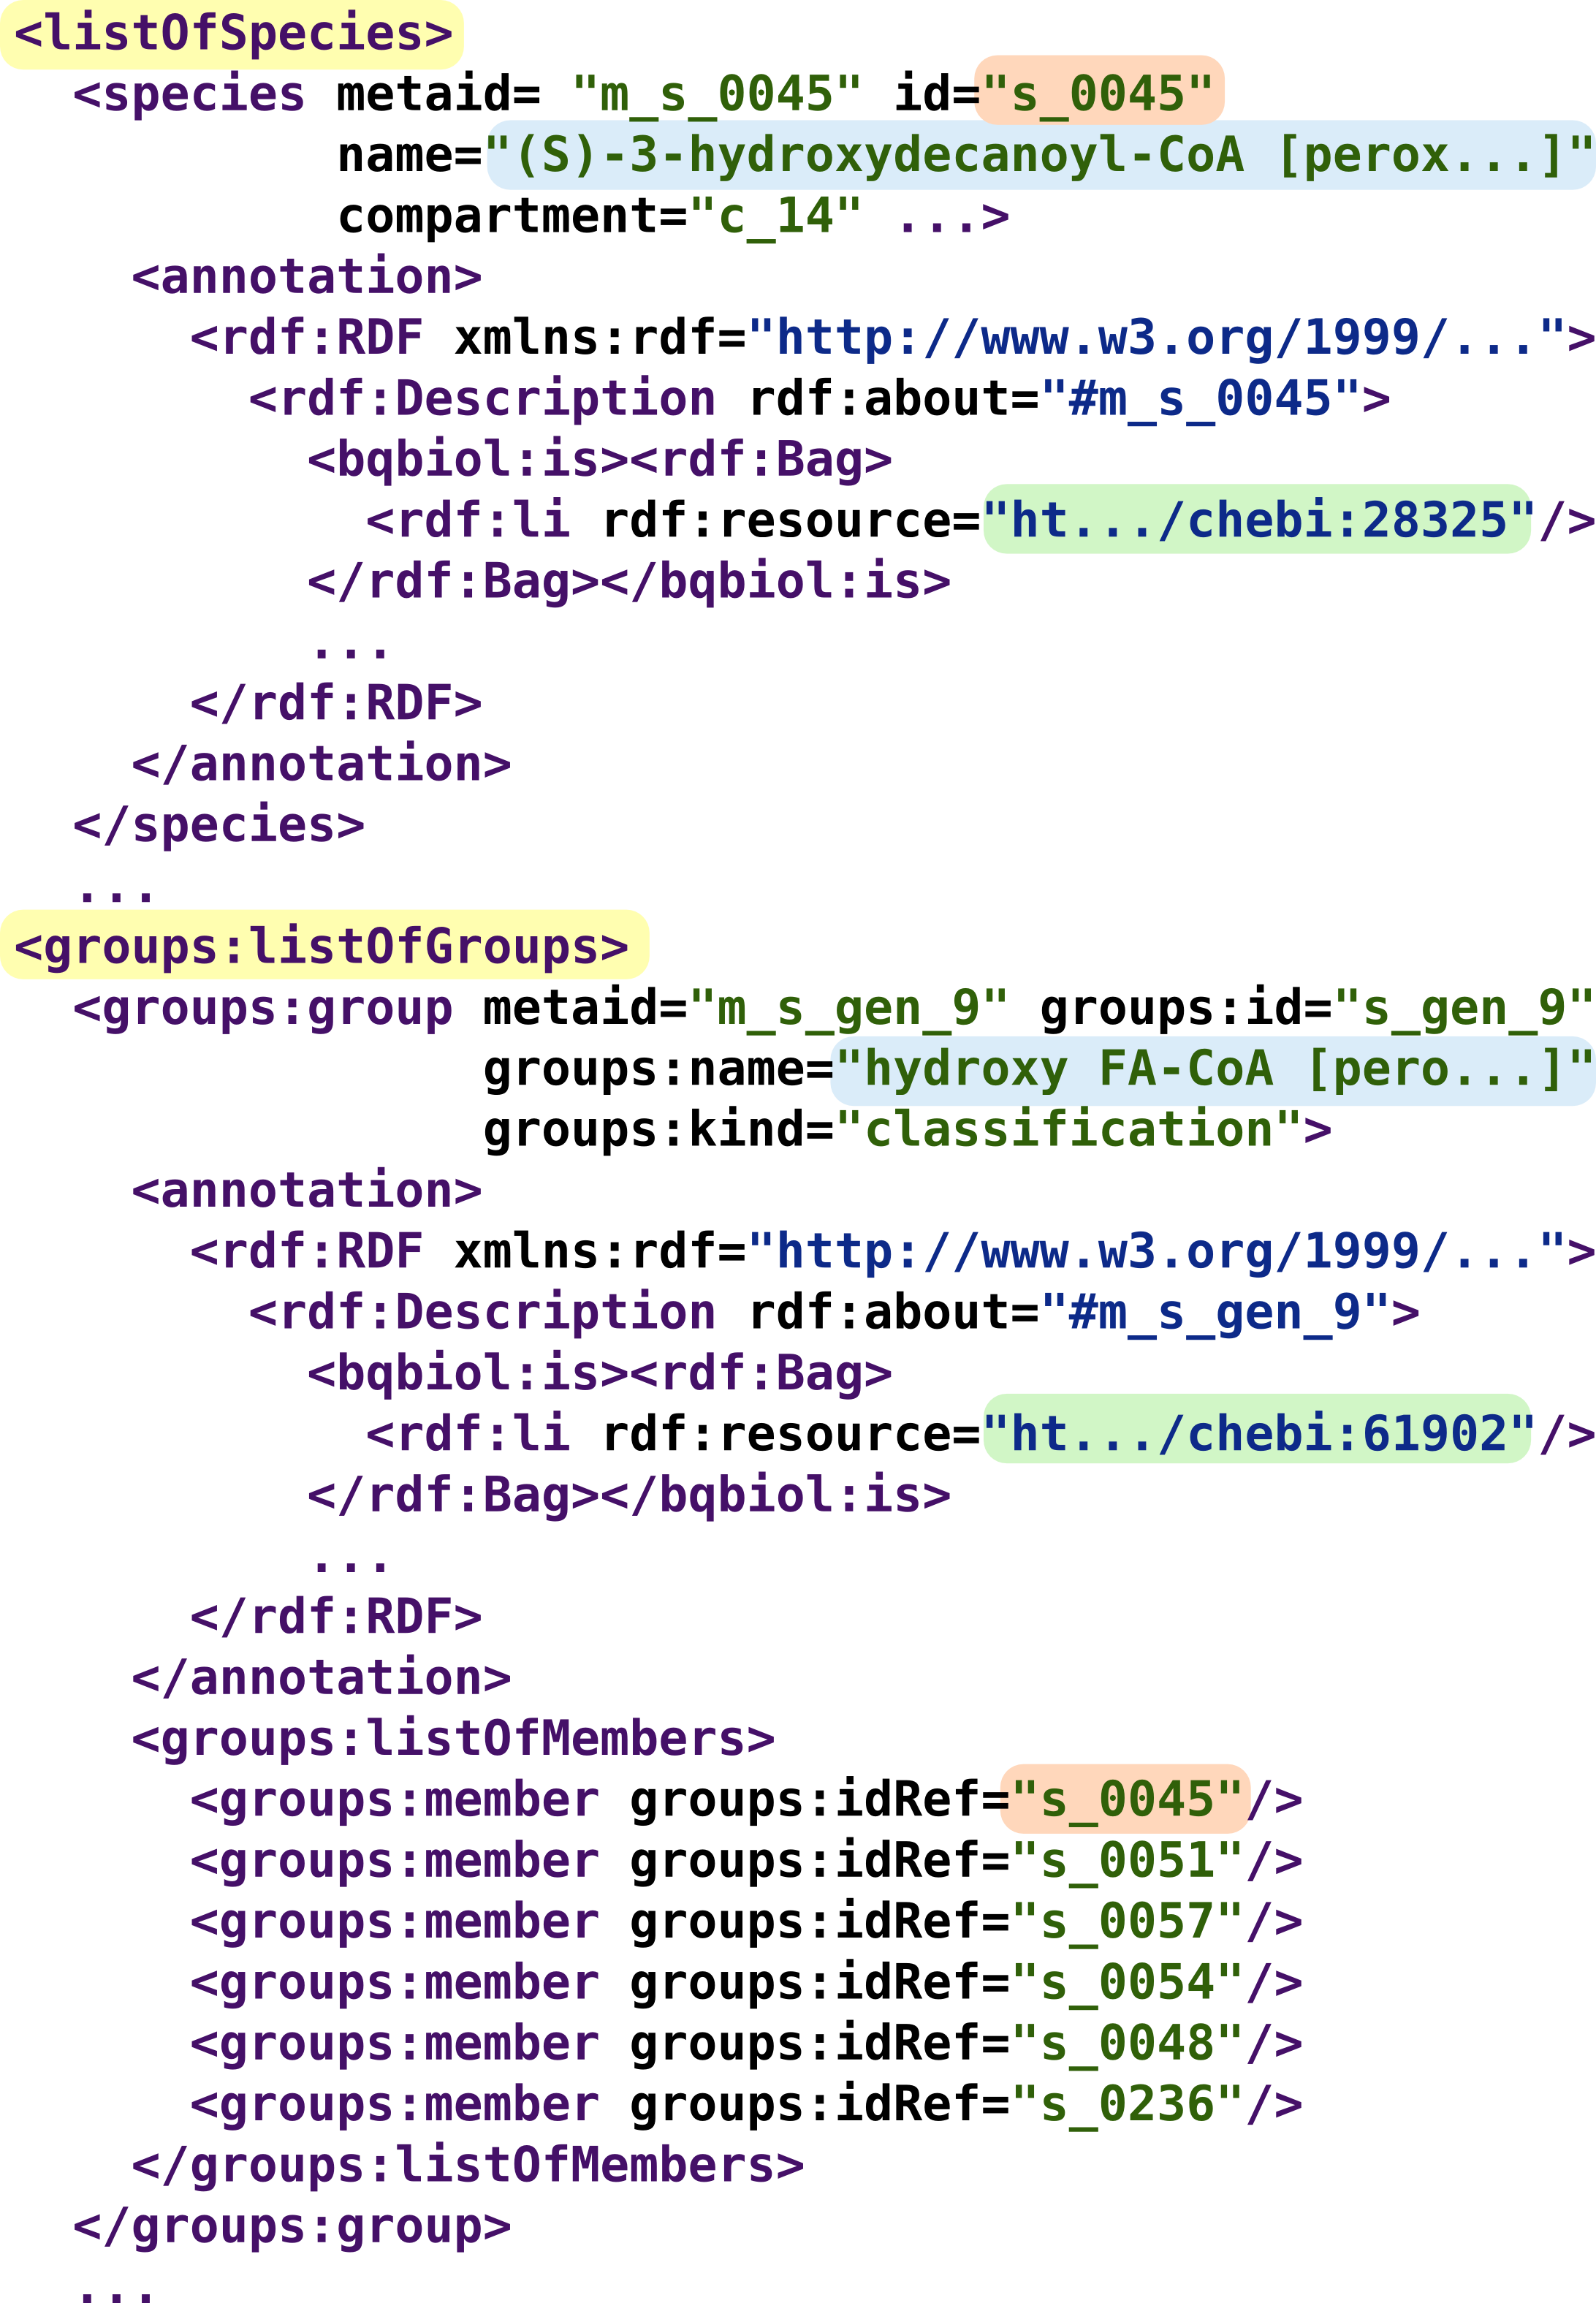
\includegraphics[scale=0.4]{groups.png}
\caption{\csentence{Representation of a generalized model in SBML level~3 version~1 format with groups extension.}
\label{fig:groups}
The output SBML file contains the initial model (including the lists of metabolites (called \emph{species} in SBML), reactions, etc.) plus the \emph{listOfGroups} section that represents non-trivial quotient metabolite and reaction sets. In the figure, a group representing a quotient metabolite set of \emph{hydroxy fatty acyl-CoAs} is shown; it includes \emph{(S)-3-hydroxydecanoyl-CoA} (s\_0045),  \emph{(S)-3-hydroxylauroyl-CoA} (s\_0051), etc. Each of those metabolites was previously declared in the \emph{listOfSpecies} section.}
\end{figure}

\begin{figure}[h!]
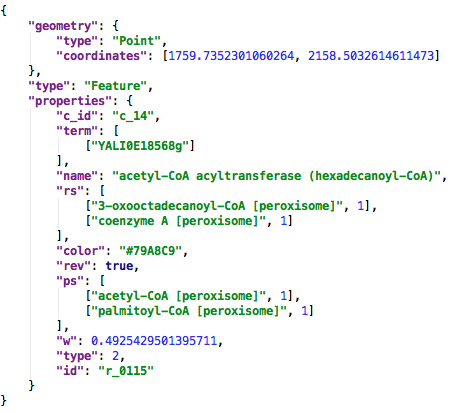
\includegraphics[scale=0.5]{figure2.png}
  \caption{\csentence{GeoJSON representation of a reaction}
  \label{fig:geojson}
      An SBML reaction is stored as a GeoJSON Point feature, with its layout coordinates encoded in the geometry section. The identifiers, labels and annotations, as well as the information on the reactant and product metabolites are stored as properties. The ``type'' property value specifies that this GeoJSON feature is a reaction.}
      \end{figure}
      
\begin{figure}[h!]
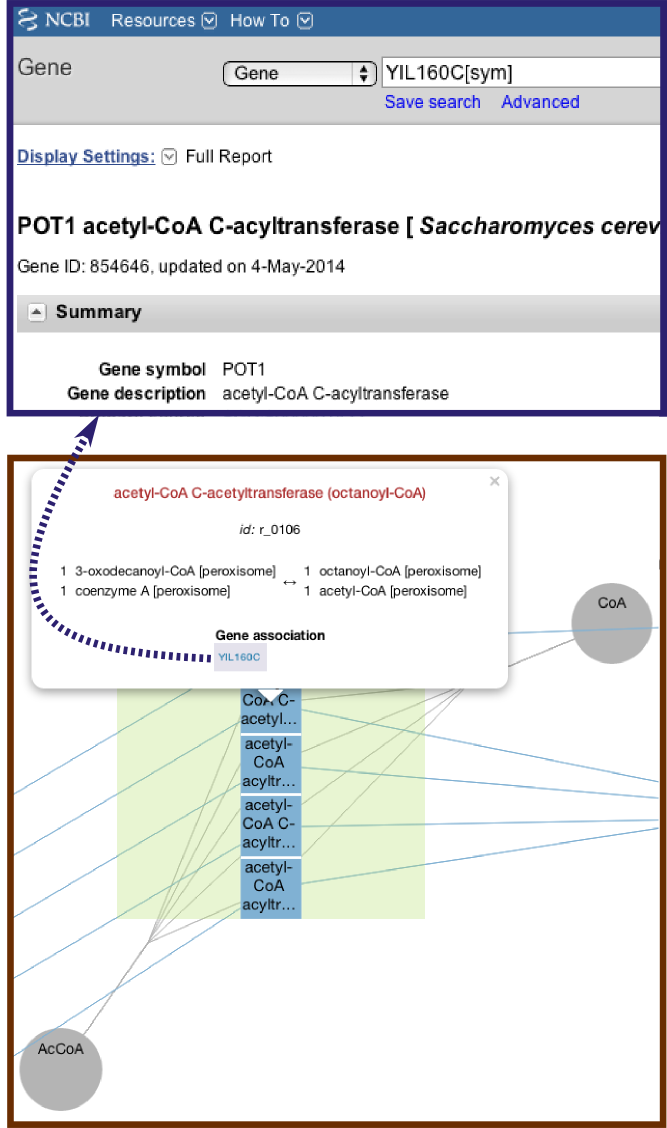
\includegraphics[scale=0.54]{figure3.png}
  \caption{\csentence{A reaction pop-up}
  \label{fig:pop_up}
      (right part) An example of a pop-up that opens when a user clicks on a reaction: It contains the information on the reaction name, identifier, reactant and product metabolites and their stoichiometries, as well as gene associations. (left part) Gene names are hyperlinks redirecting to the NCBI Gene database~\cite{NCBI}.}
      \end{figure}
      
  \begin{figure}[h!]
 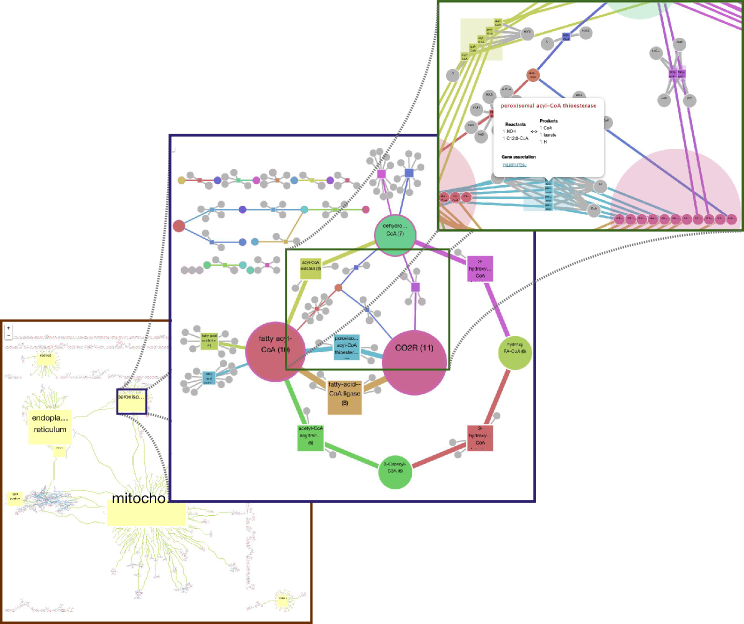
\includegraphics[scale=0.5]{figure1.png}
  \caption{\csentence{Three zoom levels}
  \label{fig:zoom_levels}
      The bottom level represents the cytoplasm compartment containing organelle compartments and transport reactions between them. The intermediate zoom shows the generalized processes in the peroxisome compartment. The most detailed view reveals the metabolites that were generalized into a \emph{straight-chain saturated fatty acid} on the previous level, e.g. \textit{dodecanoate}, and reactions they participate in.}
      \end{figure}

%%%%%%%%%%%%%%%%%%%%%%%%%%%%%%%%%%%
%%                               %%
%% Tables                        %%
%%                               %%
%%%%%%%%%%%%%%%%%%%%%%%%%%%%%%%%%%%

%% Use of \listoftables is discouraged.
%%
%\section*{Tables}
%\begin{table}[h!]
%\caption{Sample table title. This is where the description of the table should go.}
%      \begin{tabular}{cccc}
%        \hline
%           & B1  &B2   & B3\\ \hline
%        A1 & 0.1 & 0.2 & 0.3\\
%        A2 & ... & ..  & .\\
%        A3 & ..  & .   & .\\ \hline
%      \end{tabular}
%\end{table}

%%%%%%%%%%%%%%%%%%%%%%%%%%%%%%%%%%%
%%                               %%
%% Additional Files              %%
%%                               %%
%%%%%%%%%%%%%%%%%%%%%%%%%%%%%%%%%%%

\section*{Additional Files}
  \subsection*{Additional file 1 --- A video tutorial for Mimoza.}
  The video shows the main features of Mimoza, on the example of the map for the yeast consensus genome-scale metabolic network~\cite{Herrgard2008}.


\end{backmatter}
\end{document}
